\documentclass[pdflatex,compress,mathserif]{beamer}

%\usetheme[dark,framenumber,totalframenumber]{ElektroITK}
\usetheme[darktitle,framenumber,totalframenumber]{ElektroITK}

\usepackage[utf8]{inputenc}
\usepackage[T1]{fontenc}
\usepackage{lmodern}
\usepackage[bahasai]{babel}
\usepackage{amsmath}
\usepackage{amsfonts}
\usepackage{amssymb}
\usepackage{graphicx}
\usepackage{multicol}
\usepackage{framed}
\usepackage{minted}

\definecolor{LightGray}{gray}{0.95}

\usefonttheme[onlymath]{serif}

\newcommand*{\Scale}[2][4]{\scalebox{#1}{$#2$}}%

\setbeamertemplate{caption}[numbered]

\title{METODE NUMERIK}
\subtitle{Sistem Persamaan Linear}

\author{Mifta Nur Farid}

\begin{document}

\maketitle

\begin{frame}{Sistem Persamaan Linear}
    \begin{itemize}
        \item Bentuk sistem persamaan linear:
        \begin{figure}
            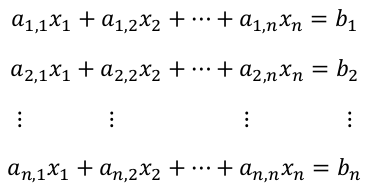
\includegraphics[width=0.7\linewidth]{./img/img01.png}
        \end{figure}
    \end{itemize}
\end{frame}

\begin{frame}{Sistem Persamaan Linear}
    \begin{itemize}
        \item Diubah ke dalam bentuk matriks:
        \begin{figure}
            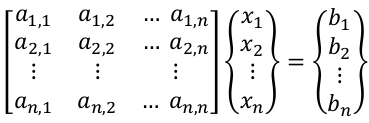
\includegraphics[width=0.7\linewidth]{./img/img02.png}
        \end{figure}
    \end{itemize}
\end{frame}

\begin{frame}{Sistem Persamaan Linear}
    \begin{itemize}
        \item Dua jenis penyelesaian
        \begin{enumerate}[a.]
            \item Metode eliminasi: Eliminasi Gauss
            \item Metode iterasi: Iterasi Jacobi dan Iterasi Gauss-Seidel
        \end{enumerate}
    \end{itemize}
\end{frame}

\begin{frame}{Iterasi Jacobi}
    \begin{itemize}
        \item Terdapat sistem persamaan linear:
        \begin{figure}
            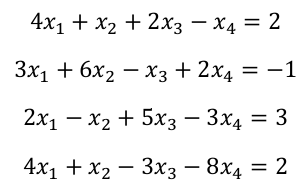
\includegraphics[width=0.5\linewidth]{./img/img03.png}
        \end{figure}
    \end{itemize}
\end{frame}

\begin{frame}{Iterasi Jacobi}
    \begin{itemize}
        \item Diubah menjadi bentuk:
        \begin{figure}
            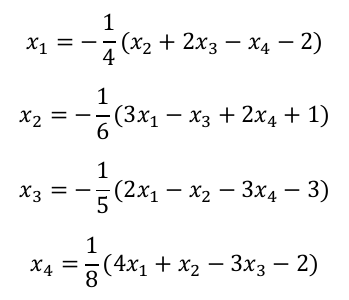
\includegraphics[width=0.5\linewidth]{./img/img04.png}
        \end{figure}
        \item Persamaan diatas digunakan sebagai persamaan dalam iterasinya, dengan nilai awalan dari masing-masing $x$
    \end{itemize}
\end{frame}

\begin{frame}{Iterasi Gauss-Seidel}
    \begin{itemize}
        \item Metode sama dengan Iterasi Jacobi, hanya saja hasil dari persamaan pertama langsung digunakan di persamaan ke dua.
        \item Kita selesaikan contoh sebelumnya dengan Metode Iterasi Gauss-Seidel.
    \end{itemize}
\end{frame}

\begin{frame}{Diagonal dominance}
    \begin{itemize}
        \item Jika bentuk sistem persamaan linearnya:
        \begin{figure}
            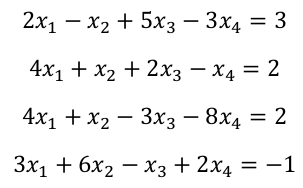
\includegraphics[width=0.5\linewidth]{./img/img05.png}
        \end{figure}
        \item Urutan persamaan perlu diubah sedemikian rupa sehingga koefisien terbesar berada di diagonal
    \end{itemize}
\end{frame}

\begin{frame}{Diagonal dominance}
    \begin{multicols}{2}
        \begin{itemize}
            \item Sebelum:
            \begin{figure}
                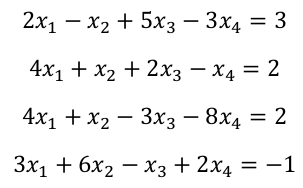
\includegraphics[width=\linewidth]{./img/img05.png}
            \end{figure}
            \columnbreak
            \item Sesudah:
            \begin{figure}
                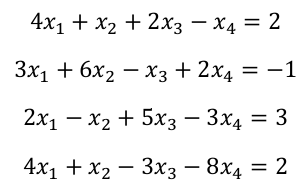
\includegraphics[width=\linewidth]{./img/img03.png}
            \end{figure}
        \end{itemize}
    \end{multicols}
    \begin{itemize}
        \item Coba kita bandingkan hasil jika tanpa perubahan urutan persamaan
    \end{itemize}
\end{frame}

\end{document}
